\documentclass[letter,10pt]{article}
\usepackage[utf8]{inputenc}
\usepackage[spanish, activeacute]{babel}
\usepackage{geometry}
\geometry{verbose,tmargin=0cm,bmargin=2cm,lmargin=2cm,rmargin=2cm,headheight=0cm,headsep=1cm,footskip=1cm}
\usepackage{graphicx}
\usepackage{fancyhdr}
\pagestyle{fancy}
\cfoot{11}
%%%%%%%%%%%%%%%%%%%%%%%%%%%%%% Textclass specific LaTeX commands.
\newcommand{\lyxaddress}[1]{
\par {\raggedright #1
\vspace{1.4em}
\noindent\par}
}

%%%%%%%%%%%%%%%%%%%%%%%%%%%%%% User specified LaTeX commands.
\date{}

\begin{document}

\title{Criptografía}


\includegraphics[scale=0.6]{logo} \hspace*{9.00cm}

\includegraphics[scale=0.5]{dsc} 
\bigskip
\begin{center}
    \Large Problema G - Código
\end{center}

\begin{flushright}
Límite de tiempo: 1 segundo
\par\end{flushright}
\bigskip

\section*{Problema}

Mau es un chico al que le encanta descifrar códigos. Recientemente un amigo suyo le contó acerca de un nuevo código que ha estado desarrollando. Este código consiste en colocar el mensaje a codificar sin espacios en una cuadrícula de $M\times N$, siendo $M$ el número de renglones y $N$ el número de columnas. Luego se rota la cuadrícula $90$ grados. Así, al leer normalmente el mensaje colocado en la cuadrícula, éste será incomprensible.

%Para hacer un poco mas fácil esta tarea, el mensaje colocado en la cuadrícula no contendrá espacios.

Un ejemplo se muestra en la siguiente imagen:

\begin{figure}[htb]
\centering
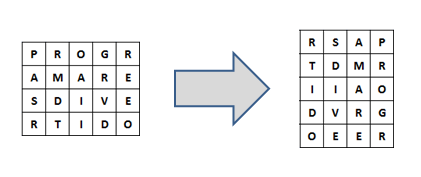
\includegraphics[width=10cm]{cr3.png}
%\caption{}
\end{figure}

Mau puede decodificar este código, pero no lo suficientemente rápido, por eso te ha pedido ayuda a ti, su amigo programador, para implementar un programa que descifre este tipo de códigos.

Tu tarea será, dado el mensaje codificado, imprimir el mensaje original que fue colocado en la cuadrícula.
$$$$
\subsection*{Entrada}

La primera línea contiene un entero $T(1\leq T\leq 50)$, el número de casos de prueba.
Para cada uno de los siguientes $T$ casos siguen 2 líneas.

La primera  de ellas contiene dos enteros $M$ y $N,(1\leq M,N\leq 50)$, que representan el número de renglones y columnas respectivamente en las que esta colocado el mensaje original.

La segunda contiene el mensaje codificado, de tamaño $M\times N$ el cual podrá estar formado de letras mayúsculas, letras minúsculas y números.  
$$$$
\subsection*{Salida}

Para cada caso imprime solo una línea que debe contener el mensaje original, con la distinción de mayúsculas y minúsculas.
\newpage
$$$$
$$$$
$$$$

\cfoot{12}

\subsection*{Entrada Ejemplo}
\begin{verbatim}
1
4 5
RSAPTDMRIIAODVRGOEER
\end{verbatim}
$$$$
\subsection*{Salida Ejemplo}
\begin{verbatim}
PROGRAMARESDIVERTIDO
\end{verbatim}

\noindent \rule[0.5ex]{1\columnwidth}{1pt}


\lyxaddress{Maximiliano Vera Luna - Grupo de Algoritmia Avanzada y Programación Competitiva}
\end{document}
